\vspace{-1em}
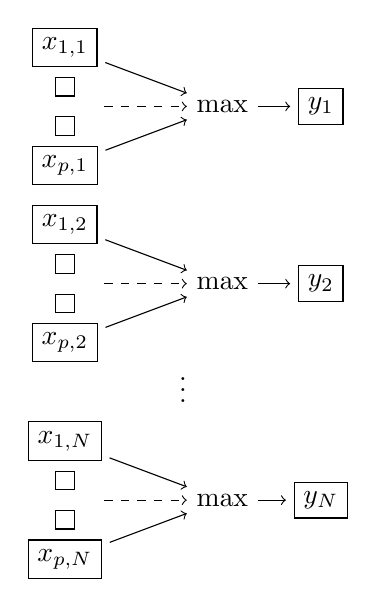
\begin{tikzpicture}[main/.style = {draw, outer sep=3pt}] 
    \node[main] (x11) at (0, 0)  {$x_{1,1}$};
    \node[main] (xx1) at (0,-0.5) {};
    \node[main] (xy1) at (0,-1) {};
    \node[main] (xp1) at (0, -1.5) {$x_{p,1}$};
    \node (y1) at (2, -0.75) {$\max$};
    \node[main] (yy1) at (3.25, -0.75) {$y_1$};

    \draw [->] (x11) -> (y1);
    \draw [->] (xp1) -> (y1);
    \draw [->, dashed] (0.5, -0.75) -> (y1);
    \draw [->] (y1) -> (yy1);


    \node[main] (x12) at (0, -2.25)  {$x_{1,2}$};
    \node[main] (xx2) at (0,-2.75) {};
    \node[main] (xy2) at (0,-3.25) {};
    \node[main] (xp2) at (0, -3.75) {$x_{p,2}$};
    \node (y2) at (2, -3) {$\max$};
    \node[main] (yy2) at (3.25, -3) {$y_2$};

    \draw [->] (x12) -> (y2);
    \draw [->] (xp2) -> (y2);
    \draw [->, dashed] (0.5, -3) -> (y2);
    \draw [->] (y2) -> (yy2);

    \node (dots) at (1.5, -4.25) {$\vdots$};


    \node[main] (x13) at (0, -5)  {$x_{1,N}$};
    \node[main] (xx3) at (0,-5.5) {};
    \node[main] (xy3) at (0,-6) {};
    \node[main] (xp3) at (0, -6.5) {$x_{p,N}$};
    \node (y3) at (2, -5.75) {$\max$};
    \node[main] (yy3) at (3.25, -5.75) {$y_N$};

    \draw [->] (x13) -> (y3);
    \draw [->] (xp3) -> (y3);
    \draw [->, dashed] (0.5, -5.75) -> (y3);
    \draw [->] (y3) -> (yy3);

\end{tikzpicture} 
